\documentclass[a4paper]{article}
\usepackage[utf8]{inputenc}
\usepackage[portuges]{babel}
\usepackage{a4wide}
\usepackage{graphicx}
\usepackage{mathtools}
\usepackage{minted}
\usepackage[hidelinks]{hyperref}

\setcounter{secnumdepth}{4}
\setcounter{tocdepth}{4}

\makeatletter
\renewcommand\paragraph{\@startsection{paragraph}{4}{\z@}%
	{-3.25ex\@plus -1ex \@minus -.2ex}%
	{1.5ex \@plus .2ex}%
	{\normalfont\normalsize\bfseries}}
\makeatother

\newminted[haskellblock]{haskell}{escapeinside=\#\#}
\newmintinline[haskell]{haskell}{escapeinside=\#\#}
\newmintedfile[haskellfile]{haskell}{}

\title{Projeto de Laboratórios de Informática I\\Grupo 44}
\author{Fábio Rafael Correia Guerra Fontes (A78650) \and Alberto Campinho Faria (A79077)}

\begin{document}

\maketitle

\begin{abstract}
Este documento consiste no relatório do projeto desenvolvido no âmbito da Unidade Curricular de Laboratórios de Informática I, visando relatar o processo de conceção e implementação das soluções aos problemas propostos pelo enunciado do projeto.
\end{abstract}

\tableofcontents

\section{Introdução}

Este documento descreve os problemas apresentados pelo enunciado do projeto elaborado no âmbito da Unidade Curricular de Laboratórios de Informática I, relatando o processo de conceção e implementação dos programas que funcionam como solução a esses problemas.

Estes problemas são todos relacionados com o puzzle \textit{Sokoban}\footnote{\url{http://www.wikipedia.org/wiki/Sokoban}}, no qual se controla um boneco numa arrecadação com o objetivo de empurrar caixas para posições predeterminadas.

O enunciado do projeto propõe um total de 6 problemas, identificados de ``Tarefa A'' a ``Tarefa F'', que podem ser resolvidos separadamente. Neste relatório abordam-se detalhadamente e em secções separadas as \emph{tarefas E e F}. As restantes tarefas são resumidas de seguida.

\bigskip

Na \emph{tarefa A} pretendia-se realizar um programa que permitisse validar se o input que lhe era fornecido cumpria os requisitos impostos pela descrição apresentada no enunciado. O input em questão representaria um tabuleiro de jogo do puzzle, juntamente com as posições iniciais do boneco e das caixas. Em caso do input recebido ser inválido, o programa deveria ainda reportar o número da linha em que fosse encontrada a primeira divergência com o formato esperado.

O objetivo da \emph{tarefa B} era o de realizar um programa que produzisse uma visualização do tabuleiro de jogo que incluisse também o boneco e as caixas, além de não apresentar paredes desnecessárias, a partir de um input no mesmo formato do input da tarefa A.

A \emph{tarefa C} propunha realizar um programa que, a partir do estado de um puzzle e de um comando que representasse um movimento do boneco, determinasse a posição do boneco após a execução desse comando. O estado do puzzle e o comando seriam obtidos a partir do input do programa, o qual estaria num formato semelhante ao formato do input das tarefas anteriores.

Com a \emph{tarefa D} pretendia-se extender o programa realizado na tarefa C, de maneira a ser possível executar uma série de comandos consecutivamente. O programa deveria devolver o número de comandos executados e ainda determinar se foi atingido um estado de fim de jogo.

\bigskip

Nas secções relativas às tarefas E e F faz-se frequentemente referência a vários tipos e funções da biblioteca \textit{Gloss}\footnote{\url{https://hackage.haskell.org/package/gloss}}, a qual é utilizada na implementação da solução de ambas essas tarefas.

\section{Tarefa E}

\subsection{Problema}

Nesta tarefa pretendia-se construir um programa que determinasse as dimensões do menor retângulo, alinhado com os eixos, que contivesse a representação visual de uma \haskell{Picture}, tipo da biblioteca \textit{Gloss} que representa uma forma ou imagem no plano.

A \haskell{Picture} deve ser lida do \texttt{stdin} com recurso à função \haskell{readPicture}, disponível na biblioteca \textit{GlossExtras}, a qual foi fornecida juntamente com o enunciado.

O valor do tipo \haskell{Picture} em questão pode ter sido construído através de um dos seguintes construtores: \haskell{Blank}, \haskell{Polygon}, \haskell{Line}, \haskell{Circle}, \haskell{Bitmap}, \haskell{Color}, \haskell{Translate}, \haskell{Rotate}, \haskell{Scale} ou \haskell{Pictures}. (Note-se que são ignorados os construtores \haskell{ThickCircle}, \haskell{Arc}, \haskell{ThickArc} e \haskell{Text}.)

\subsection{Conceção da Solução}
\label{sec:tarefaEconc}

Tem de se ter em conta três categorias principais de construtores do tipo \haskell{Picture}:

\begin{itemize}
	\item Construtores que definem formas ``básicas'' ou nenhuma forma de todo: \haskell{Blank}, \haskell{Polygon}, \haskell{Line}, \haskell{Circle} e \haskell{Bitmap};
	\item Construtores que transformam formas já existentes: \haskell{Color}, \haskell{Translate}, \haskell{Rotate} e \haskell{Scale};
	\item Construtores que juntam várias formas já existentes: \haskell{Pictures}.
\end{itemize}

O menor retângulo, alinhado com os eixos, que contém uma \haskell{Picture} corresponde ao menor retângulo que contém todos os pontos da representação visual dessa \haskell{Picture}. Assim, reduz-se o problema ao cálculo das maiores e menores coordenadas de todos os pontos que uma \haskell{Picture} contém.

\bigskip

Considere-se a \haskell{Picture} definida da seguinte forma:

\begin{haskellblock}
pic :: Picture
pic = Rotate 30 #\$# Polygon [(0,0), (1,2), (2,0)]
\end{haskellblock}

Se se começasse por converter o valor \haskell{Polygon [(0,0), (1,2), (2,0)]} no retângulo que o envolve, aplicando depois a rotação a esse retângulo, o resultado obtido não seria correto, já que o novo retângulo não estaria sequer alinhado com os eixos. Verifica-se assim que a conversão de uma \haskell{Picture} no retângulo que a envolve não pode ser feita imediatamente, nem aplicada recursivamente a construtores que transformem ou juntem outros valores do tipo \haskell{Picture}.

Uma solução possível seria a de criar um tipo auxiliar intermédio capaz de representar as mesmas formas que uma \haskell{Picture}, mas que consiga também representar formas transformadas ``não recursivamente''. Um valor do tipo \haskell{Picture} seria primeiro convertido num valor desse tipo auxiliar, e só depois se faria o cálculo do retângulo envolvente da \haskell{Picture}.

Formas constituídas por um conjunto de vértices (i.e. valores dos construtores \haskell{Polygon}, \haskell{Line} ou \haskell{Bitmap}) poderiam então ser armazenadas através de uma lista dos seus vértices, já que as coordenadas extremas dessas formas correspondem sempre a coordenadas de vértices. Transformações sobre essas formas (i.e. valores dos construtores \haskell{Color}, \haskell{Translate}, \haskell{Rotate} e \haskell{Scale} que contenham formas constituídas por um conjunto de vértices) seriam facilmente convertidas em valores do tipo intermédio efetuando primeiro a conversão da forma a ser transformada num valor desse tipo intermédio, e de seguida aplicando a transformação em questão a todos os seus vértices; o construtor \haskell{Color} não resultaria, naturalmente, em nenhuma transformação dos vértices.

Assim, o retângulo envolvente do valor \haskell{pic} definido anteriormente seria calculado da seguinte forma:

\begin{enumerate}
	\item Transformar o valor \haskell{Polygon [(0,0), (1,2), (2,2)]} num valor do tipo intermédio em questão, que neste caso seria constituído por uma lista de vértices;
	\item Aplicar a rotação a todos esses vértices;
	\item Calcular o retângulo envolvente do polígono, determinando as coordenadas de menor e maior valor, ao longo dos dois eixos, de todos os vértices do polígono.
\end{enumerate}

Valores do tipo \haskell{Picture} sem representação visual (e.g. \haskell{Blank} ou \haskell{Polygon []}) poderiam ser representados similarmente através de uma lista de vértices vazia.

Formas definidas através do construtor \haskell{Circle} não poderiam ser representadas (de forma exata) como uma lista de vértices. Além disso, ao serem aplicadas transformações a circunferências, existiria a possibilidade de estas se transformarem em elipses.

\bigskip

Uma possibilidade seria a de representar elipses (sendo a circunferência um caso especial destas) através das coordenadas do seu centro, do comprimento dos semieixos principal e secundário e do ângulo que o semieixo principal faria com o eixo \(Ox\) (cf. figura \ref{fig:ellipse}).

\begin{figure}[ht]
	\centering
	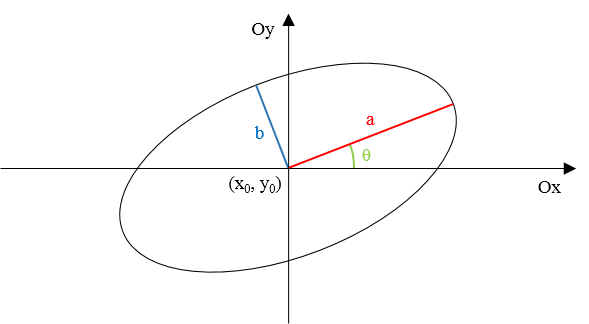
\includegraphics{images/ellipse.png}
	\caption{Elipse centrada na origem.}
	\label{fig:ellipse}
	\smallskip\small
	\((x_0, y_0)\) - coordenadas do centro; \(a\) - comprimento do semieixo principal; \(b\) - comprimento do semieixo secundário; \(\theta\) - ângulo do semieixo principal em relação ao eixo \(Ox\).
\end{figure}

Os limites do retângulo envolvente de uma elipse descrita desta forma seriam dados pelas seguintes expressões (cf. \url{http://math.stackexchange.com/a/91304}):

\[ x = x_0 \pm \sqrt{a^2 \cos^2 \theta + b^2 \sin^2 \theta} \]
\[ y = y_0 \pm \sqrt{a^2 \sin^2 \theta + b^2 \cos^2 \theta} \]

As coordenadas ao longo do eixo \(Ox\) das arestas esquerda e direita do retângulo seriam dadas, respetivamente, pelo valores menor e maior de \(x\); as coordenadas ao longo do eixo \(Oy\) das arestas inferior e superior do retângulo seriam dadas, respetivamente, pelo valores menor e maior de \(y\).

Para descrever uma circunferência centrada na origem e de raio \(r\), construir-se-ia então uma elipse com os parâmetros \(x_0 = y_0 = 0,\ a = b = r,\ \theta = 0\).

Aplicar uma translação a uma elipse resumir-se-ia a transladar o seu centro; aplicar uma rotação implicaria aplicar essa transformação ao seu centro e adicionar o ângulo da rotação ao parâmetro \(\theta\); aplicar uma transformação de escala \emph{uniforme} seria equivalente a aplicar essa transformação ao seu centro e ao comprimento de ambos os seus semieixos. No entanto, não foi encontrada forma de aplicar uma transformação de escala \emph{não uniforme} a uma elipse descrita por estes parâmetros.

\bigskip

Uma forma alternativa de representar elipses (sendo a circunferência um caso especial destas) seria através de uma matriz que transformasse a circunferência unitária (circunferência de centro na origem e raio 1) na elipse em questão. Uma matriz resultante da combinação de várias transformações de translação, rotação e escala é capaz de representar assim qualquer elipse.

Para este fim, utilizar-se-iam matrizes quadradas de ordem 3, as quais são capazes de representar qualquer das transformações supracitadas. Para combinar transformações, recorrer-se-ia ao produto de matrizes da forma \(M = BA\), onde \(M\) corresponderia à matriz da transformação cuja aplicação seria equivalente à aplicação da transformação de matriz \(A\) seguida da aplicação da transformação de matriz \(B\). Apresentam-se a seguir as formas das matrizes que correspondem às três transformações em questão.

\begin{figure}[ht]

	\centering

	Matriz de translação associada à translação \(\vec{t} = (t_x, t_y)\):

	\medskip

	\(
	\begin{bmatrix}
		0 & 0 & t_x \\
		0 & 0 & t_y \\
		0 & 0 &   1
	\end{bmatrix}
	\)

	\bigskip

	Matriz de rotação associada ao ângulo \(\theta\):

	\medskip

	\(
	\begin{bmatrix}
		cos\ \theta & -sin\ \theta & 0 \\
		sin\ \theta &  cos\ \theta & 0 \\
		          0 &            0 & 1
	 \end{bmatrix}
	\)

	\bigskip

	Matriz de transformação de escala associada à escala \(s = (s_x, s_y)\):

	\medskip

	\(
	\begin{bmatrix}
		s_x &   0 & 0 \\
		0   & s_y & 0 \\
		0   &   0 & 1
	 \end{bmatrix}
	\)

\end{figure}

Os limites do retângulo envolvente de uma elipse descrita desta forma seriam dados pelas seguintes expressões, considerando \(M = (m_{i,j})\) correspondente à matriz de transformação que constrói a elipse a partir da circunferência unitária (cf. \url{http://www.stackoverflow.com/q/24746834}):

\[ x = m_{1,3} \pm \sqrt{m_{1,1}^2 + m_{1,2}^2} \]
\[ y = m_{2,3} \pm \sqrt{m_{2,1}^2 + m_{2,2}^2} \]

As coordenadas ao longo do eixo \(Ox\) das arestas esquerda e direita do retângulo seriam dadas, respetivamente, pelo valores menor e maior de \(x\); as coordenadas ao longo do eixo \(Oy\) das arestas inferior e superior do retângulo seriam dadas, respetivamente, pelo valores menor e maior de \(y\).

Para descrever uma circunferência centrada na origem e de raio \(r\), construir-se-ia uma matriz de escala associada à escala \(s = (r,r)\), ou seja:

\[
\begin{bmatrix}
	r & 0 & 0 \\
	0 & r & 0 \\
	0 & 0 & 1
 \end{bmatrix}
\]

Aplicar uma transformação de translação, rotação ou escala (\emph{uniforme ou não uniforme}) a uma elipse, passaria apenas por multiplicar a matriz associada com essa transformação pela matriz da elipse, segundo a expressão \(M' = TM\), onde \(T\) corresponde à matriz da transformação, \(M\) corresponde à matriz da elipse a transformar e \(M'\) corresponde à matriz da elipse transformada.

A implementação da solução a esta tarefa, a qual será abordada na secção seguinte (secção \ref{sec:tarefaEimpl}), segue esta mesma estratégia.

\bigskip

Figuras que consistem de um conjunto de outras figuras (i.e. valores do tipo \haskell{Picture} e do constructor \haskell{Pictures}) seriam armazenadas, simplesmente, como uma lista de figuras. As coordenadas extremas do retângulo, alinhado com os eixos, envolvente dessa figura, corresponderiam às coordenadas extremas maiores e menores dos retângulos envolventes de cada subfigura.

\subsection{Implementação da Solução}
\label{sec:tarefaEimpl}

\emph{Ao longo desta secção são utilizados vários tipos e funções auxiliares, cuja definição pode ser consultada no anexo \ref{app:tarefaEaux}.}

\bigskip

Começou-se por elaborar o tipo intermédio descrito na secção anterior (secção \ref{sec:tarefaEconc}), responsável por descrever figuras individuais não recursivamente e conjuntos de figuras através de uma lista de figuras. A definição desse tipo, de nome \haskell{Shape}, é a seguinte:

\begin{haskellblock}
data Shape
    = ShapePoints  [Vector]
    | ShapeEllipse Matrix
    | ShapeList    [Shape]
\end{haskellblock}

Os construtores deste tipo têm as seguintes finalidades:

\begin{itemize}
	\item \haskell{ShapePoints} - representa uma forma que pode ser descrita através de uma lista de vértices (e.g. um polígono);
	\item \haskell{ShapeEllipse} - descreve uma elipse através de uma matriz que transforma a circunferência unitária nessa elipse; é também utilizado para representar circunferências;
	\item \haskell{ShapeList} - representa um conjunto de figuras, através de uma lista de valores do mesmo tipo.
\end{itemize}

\bigskip

De seguida, elaborou-se uma função de nome \haskell{pictureToShape}, responsável por converter valores do tipo \haskell{Picture} em valores do tipo \haskell{Shape}. A implementação da função é a seguinte:

\begin{haskellblock}
pictureToShape :: Picture -> Shape
pictureToShape Blank               = ShapePoints []
pictureToShape (Polygon pts)       = ShapePoints pts
pictureToShape (Line pts)          = ShapePoints pts
pictureToShape (Circle r)          = ShapeEllipse #\$# scalingMatrix (r,r)
pictureToShape (Bitmap w h _ _)    =
    ShapePoints [(-hw,-hh), (hw,-hh), (hw,hh), (-hw,hh)]
    where
        hw = (fromIntegral w) / 2
        hh = (fromIntegral h) / 2
pictureToShape (Color _ pic)       = pictureToShape pic
pictureToShape (Translate x y pic) = translateShape (x,y) (pictureToShape pic)
pictureToShape (Rotate r pic)      = rotateShape th (pictureToShape pic)
    where th = degToRad (-r)
pictureToShape (Scale sx sy pic)   = scaleShape (sx,sy) (pictureToShape pic)
pictureToShape (Pictures pics)     = ShapeList #\$# map pictureToShape pics
\end{haskellblock}

Ao valor \haskell{Blank} fez-se corresponder o valor \haskell{ShapePoints []}, descrevendo-se assim uma figura sem representação visual; seria equivalente fazer-lhe corresponder o valor \haskell{ShapeList []}. A valores que descrevem figuras pelos seus vértices, fez-se corresponder valores do construtor \haskell{ShapePoints} com os mesmo vértices associados. Para os construtores \haskell{Polygon} e \haskell{Line}, este processo é imediato; no caso do construtor \haskell{Bitmap}, têm de ser calculados os vértices do retângulo envolvente do bitmap em questão. Valores da forma \haskell{Circle r} são convertidos no valor \haskell{ShapeEllipse #\$# scalingMatrix}\\\haskell{(r,r)}, de acordo com o descrito na secção anterior.

A conversão de valores de construtores que transformam uma figura já existente passa por primeiro converter a \haskell{Picture} a ser transformada numa \haskell{Shape}, e de seguida aplicar a transformação em questão à \haskell{Shape}. O construtor \haskell{Color} não altera a figura. Os construtores \haskell{Translate}, \haskell{Rotate} e \haskell{Scale} delegam o processo de transformação para as funções \haskell{translateShape}, \haskell{rotateShape} e \haskell{scaleShape}, respetivamente, as quais serão descritas a seguir.

Para converter um conjunto de figuras descrito por um valor do construtor \haskell{Pictures}, faz-se primeiro a conversão de cada subfigura para uma \haskell{Shape}, juntando-se todas as figuras resultantes através do construtor \haskell{ShapeList}.

\bigskip

A função \haskell{translateShape} aplica uma translação a uma \haskell{Shape}. Se o valor for do construtor \haskell{ShapePoints}, o vetor associado à translação é somado a cada vértice; se o valor for do construtor \haskell{ShapeEllipse}, a matriz da nova elipse corresponde ao produto da matriz associada à translação em questão com a matriz da elipse a transformar; se o valor for do construtor \haskell{ShapeList}, a função é aplicada recursivamente a todas as subfiguras. Segue-se a definição desta função:

\begin{haskellblock}
translateShape :: Vector -> Shape -> Shape
translateShape t (ShapePoints pts)  = ShapePoints #\$# map (|+| t) pts
translateShape t (ShapeEllipse m)   = ShapeEllipse #\$# translationMatrix t `matMul` m
translateShape t (ShapeList shapes) = ShapeList #\$# map (translateShape t) shapes
\end{haskellblock}

A função \haskell{rotateShape} aplica uma rotação a uma \haskell{Shape}. Se o valor for do construtor \haskell{ShapePoints}, a rotação é aplicada a cada vértice; se o valor for do construtor \haskell{ShapeEllipse}, a matriz da nova elipse corresponde ao produto da matriz associada à rotação em questão com a matriz da elipse a transformar; se o valor for do construtor \haskell{ShapeList}, a função é aplicada recursivamente a todas as subfiguras. Segue-se a definição desta função:

\begin{haskellblock}
rotateShape :: Float -> Shape -> Shape
rotateShape r (ShapePoints pts)  = ShapePoints #\$# map (rotateV r) pts
rotateShape r (ShapeEllipse m)   = ShapeEllipse #\$# rotationMatrix r `matMul` m
rotateShape r (ShapeList shapes) = ShapeList #\$# map (rotateShape r) shapes
\end{haskellblock}

A função \haskell{scaleShape} aplica uma transformação de escala a uma \haskell{Shape}. Se o valor for do construtor \haskell{ShapePoints}, cada vértice é multiplicado componente a componente pelo vetor associado à escala; se o valor for do construtor \haskell{ShapeEllipse}, a matriz da nova elipse corresponde ao produto da matriz associada à transformação de escala em questão com a matriz da elipse a transformar; se o valor for do construtor \haskell{ShapeList}, a função é aplicada recursivamente a todas as subfiguras. Segue-se a definição desta função:

\begin{haskellblock}
scaleShape :: Vector -> Shape -> Shape
scaleShape s (ShapePoints pts)  = ShapePoints #\$# map (s |*|) pts
scaleShape s (ShapeEllipse m)   = ShapeEllipse #\$# scalingMatrix s `matMul` m
scaleShape s (ShapeList shapes) = ShapeList #\$# map (scaleShape s) shapes
\end{haskellblock}

\bigskip

De seguida, definiu-se a função \haskell{shapeBounds}, responsável por calcular o menor retângulo, alinhado com os eixos, que contenha a representação visual de um dado valor do tipo \haskell{Shape}. A seguinte lista descreve o comportamento da função para valores de diferentes construtores:

\begin{itemize}
	\item \haskell{ShapePoints} - as coordenadas, ao longo dos eixos correspondentes, das arestas do retângulo são dadas pelas coordenadas máximas e mínimas dos vários vértices da figura;
	\item \haskell{ShapeEllipse} - as coordenadas, ao longo dos eixos correspondentes, das arestas do retângulo são calculadas a partir da matriz que descreve a elipse, através das expressões apresentadas na secção anterior (secção \ref{sec:tarefaEconc});
	\item \haskell{ShapeList} - o retângulo que envolve a figura corresponde ao menor retângulo, alinhado com os eixos, que contém os retângulos de cada subfigura.
\end{itemize}

Se a forma não tiver uma representação visual, é devolvido o valor \haskell{Nothing}. Em caso contrário, é devolvido o valor \haskell{Just rect}, onde \haskell{rect} corresponde ao menor retângulo, alinhado com os eixos, que contém a figura. Segue-se a implementação da função em questão:

\begin{haskellblock}
shapeBounds :: Shape -> Maybe Rect
shapeBounds (ShapePoints [])  = Nothing
shapeBounds (ShapePoints pts) =
    Just #\$# Rect
        (minimum #\$# map fst pts)
        (minimum #\$# map snd pts)
        (maximum #\$# map fst pts)
        (maximum #\$# map snd pts)
shapeBounds (ShapeEllipse m) = Just #\$# Rect xMin yMin xMax yMax
    where
        xCenter = m `matGet` (1,3)
        yCenter = m `matGet` (2,3)
        xOffset = sqrt #\$# (m `matGet` (1,1))^2 + (m `matGet` (1,2))^2
        yOffset = sqrt #\$# (m `matGet` (2,1))^2 + (m `matGet` (2,2))^2
        xMin = xCenter - xOffset
        xMax = xCenter + xOffset
        yMin = yCenter - yOffset
        yMax = yCenter + yOffset
shapeBounds (ShapeList shapes) = joinRects #\$# mapMaybe shapeBounds shapes
\end{haskellblock}

\bigskip

Definiu-se ainda a função \haskell{pictureBounds}:

\begin{haskellblock}
pictureBounds :: Picture -> Maybe Rect
pictureBounds = shapeBounds . pictureToShape
\end{haskellblock}

A partir destas funções, é possível definir a função principal do programa, a qual recebe uma \haskell{Picture} e devolve um valor do tipo \haskell{(Float, Float)} que representa as dimensões do menor retângulo, alinhado com os eixos, que contém a figura em questão:

\begin{haskellblock}
tarefaE :: Picture -> (Float, Float)
tarefaE pic = maybe (0,0) rectSize (pictureBounds pic)
\end{haskellblock}

No caso de a \haskell{Picture} não ter representação visual, é devolvido o valor \haskell{(0,0)}.

\subsection{Testes}

Para testar a validade do programa, foram elaborados testes de três tipos:

\begin{itemize}
	\item Verificação de pares de input-output sobre o programa (black-box testing): o programa é executado com diferentes inputs, verificando-se se o seu output corresponde ao output esperado para o input correspondente.
	\item Verificação de pares de input-output sobre funções individuais: através da utilização da biblioteca \textit{HUnit}\footnote{\url{http://hunit.sourceforge.net}}, definiram-se vários testes de verificação da correspondência do output de várias funções com determinados inputs.
	\item Verificação de propriedades de funções: recorrendo à biblioteca \textit{QuickCheck}\footnote{\url{https://github.com/nick8325/quickcheck}}, criaram-se vários testes para a verificação de diversas propriedades de várias funções.
\end{itemize}

No total, definiram-se 62 testes de black-box testing, 21 testes através da biblioteca \textit{HUnit} e 8 testes através da biblioteca \textit{QuickCheck}. O programa passa em todos.

O programa foi também submetido na plataforma \textit{mooshak}, como indicado pelo enunciado do projeto, tendo passado em todos os testes automáticos dessa mesma plataforma.

\section{Tarefa F}

\subsection{Problema}

Nesta tarefa pretendia-se desenvolver um programa que permitisse jogar o \textit{Sokoban} através de uma interface gráfica, tirando partido das funcionalidades da biblioteca \textit{Gloss}. Como ponto de partida, entendia-se que o programa deveria oferecer funcionalidades semelhantes ao encontrado em \url{sokoban.info}.

O mapa de jogo deveria ser lido a partir do \texttt{stdin}, sendo o seu formato equivalente ao formato do input das tarefas A, B, C e D. De seguida, deveria ser aberta uma janela que permitisse a interação do utilizador com o jogo, associando comandos a teclas específicas.

\subsection{Planificação e Objetivos}

Começou-se por planificar o jogo e definir as suas funcionalidades principais e objetivos que queríamos cumprir. Nesta secção apresentam-se, de forma geral, esses objetivos, os quais serão descritos em maior detalhe na próxima secção (secção \ref{sec:tarefaFimpl}).

\bigskip

De modo a diversificar o jogo e a disponibilizar vários modos de jogo, decidiu-se incluir vários personagens, os quais teriam capacidades diferentes que acabariam por alterar a dinâmica do jogo. Segue-se uma lista dos quatro personagens disponíveis na versão final do jogo:

\begin{itemize}
	\item \emph{``Sokoban''} - personagem clássica do jogo \textit{Sokoban}; consegue empurrar apenas uma caixa em simultâneo; não possui nenhuma habilidade especial;
	\item \emph{``The Hulk''} - consegue empurrar até 3 caixas em simultâneo;
	\item \emph{``Captain Hook''} - tem a habilidade de puxar caixas; apenas consegue empurrar uma caixa em simultâneo;
	\item \emph{``Teleporting Girl''} - tem a habilidade de se teleportar para locais por onde já passou.
\end{itemize}

Para permitir a escolha, pelo utilizador, do personagem a ser utilizado para jogar, elaborou-se um menu inicial que permite a seleção do personagem. Este menu exibe o título do jogo e disponibiliza um seletor de personagem e botões interativos que permitem, ao utilizador, avançar para o jogo com o personagem selecionado ou sair do jogo. Estes elementos interativos da interface do utilizador permitem todos a interação através do rato ou do teclado.

\bigskip

Depois da escolha do personagem, o utilizador passa à fase do jogo.

Decidimos disponibilizar a capacidade para jogar vários níveis consecutivamente. Os vários níveis podem ser especificados através do \texttt{stdin}, separados por linhas vazias, ou através de argumentos do programa que especificam ficheiros e/ou diretorias com ficheiros de níveis.

Permitiu-se também a especificação de comandos, juntamente com a descrição de cada nível, que fazem com que o personagem se mova automaticamente de acordo com esses comandos, no início de cada nível, antes de permitir que o utilizador o controle.

Adicionou-se a capacidade de o utilizador anular jogadas efetuadas, permitindo também recomeçar o nível atual. O utilizador é também capaz de desistir do nível atual, podendo avançar para o próximo nível ou voltar ao menu de seleção do personagem. 

Nesta fase encontra-se na janela uma representação visual do mapa de jogo, a qual inclui o personagem que o utilizador controla e as caixas. Também foi incluido um painel de informação que exibe o número do nível atual, o número total de níveis disponíveis, o número de passos efetuados pelo personagem, e o tempo decorrido desde o início do nível atual. Existe um painel de botões que permite anular uma jogada, recomeçar o nível atual, ou voltar ao menu de seleção do personagem.

Para a representação gráfica do tabuleiro de jogo, decidiu-se elaborar um sistema que determina a imagem correspondente a uma determinada célula do tabuleiro não apenas a partir dessa célula, mas também a partir das células que a rodeiam. Esta imagem é também escolhida aleatoriamente de entre uma lista de imagens com probilidades diferentes. Existem também diversos aspetos visuais (chamados \emph{temas}), escolhidos aleatoriamente para cada nível. Estas funcionalidades permitiram melhorar o aspeto gráfico do jogo.

Decidiu-se incluir animações para o personagem e para as caixas. O personagem, dependendo da direção para a qual está virado, da natureza do seu movimento (e.g. se está a andar ou a agarrar uma caixa) e da fase do seu movimento (e.g. se se encontra no início ou a meio do seu movimento), é desenhado com imagens diferentes. Tanto o personagem como as caixas mudam de posição gradualmente ao longo do seu movimento.

\bigskip

Toda a interface gráfica, quer na fase do menu principal, quer na fase do jogo, é automaticamente redimensionada de forma a ocupar o máximo de espaço na janela e ser totalmente visível.

Como já referido, todos os elementos interativos da interface do utilizador permitem a interação através do rato e do teclado.

Para desenhar texto, devido às limitações do sistema disponibilizado pela biblioteca \textit{Gloss}, o qual não permite a especificação exata do tamanho ou da posição do texto, decidiu-se elaborar um sistema específico para este fim.

\subsection{Implementação}
\label{sec:tarefaFimpl}

O programa foi implementado em vários módulos. A hierarquia de módulos resultante e as dependências entre estes podem ser consultados no anexo \ref{app:tarefaFmodulos}. O módulo inicial do programa é o módulo \haskell{Sokoban}.

\subsubsection{Recursos externos}

Ao longo de todo o programa existe a necessidade de utilizar recursos externos, como por exemplo imagens. De modo a perimitir um acesso fácil e uniforme, por todas as partes do programa, a esses recursos externos, foi criado o módulo \haskell{Sokoban.Assets}. 

\bigskip

São utilizados dois tipos principais de recursos, os quais denominamos \emph{bitmap} e \emph{sprite}. Ambos são construidos a partir de ficheiros bitmap.

Um \emph{bitmap} consiste apenas de uma imagem, carregada a partir de um ficheiro bitmap, e pode ser utilizado diretamente como um valor do tipo \haskell{Picture}.

Um \emph{sprite} consiste de um conjunto de imagens, cada uma com uma probabilidade associada; a soma das probabilidades de todas as imagens deve ser de 100\%. Isto permite escolher aleatoriamente uma das imagens do sprite (o que é útil, por exemplo, para adicionar alguma divesidade ao aspeto dos tabuleiros de jogo). Cada imagem que constitui um sprite é carregada de um ficheiro bitmap individual; a probabilidade associada com cada imagem é codificada no nome desse ficheiro (para mais informações, cf. documentação do código).

\bigskip

O módulo exporta o tipo abstrato \haskell{Assets}, capaz de armazenar todos os recursos que o programa utiliza, juntamente com a função \haskell{load :: IO Assets}, a qual permite carregar esses mesmos recursos.

\bigskip

A interface do utilizador depende de vários bitmaps, os quais estão localizados, relativamente ao executável do programa, na diretoria \texttt{assets/ui/}. Todos os ficheiros bitmap que se encontram nessa diretoria são carregados.

O módulo exporta a função \haskell{uiBitmap :: String -> Assets -> Picture}, a qual permite, através do nome de um certo bitmap da interface do utilizador, aceder a esse bitmap.

\bigskip

Para desenhar os personagens que o utilizador controla durante o jogo, são necessárias várias imagens para cada fase da animação, ação que está a realizar e direção para onde o personagem está virado. Estas imagens são carregadas a partir de todas as diretorias que se encontram, relativamente ao executável do programa, na diretoria \texttt{assets/players/}.

O módulo exporta a função \haskell{playerBitmap :: String -> String -> Assets -> Picture} que a partir do nome da diretoria (relativa à diretoria \texttt{assets/players/}) e do nome de um bitmap, permite aceder a esse bitmap.

\bigskip

O tabuleiro de jogo e as caixas podem ter vários aspetos. Quando um nível é criado, é escolhido um aspeto aleatoriamente. A estes aspetos chamamos \emph{temas}. Um tema é um conjunto de sprites que são utilizados para desenhar as células do tabuleiro e as caixas. Às imagens utilizadas nas células do tabuleiro chamamos \emph{tiles}. As tiles e imagens das caixas de cada tema são carregadas a partir de todas as diretorias que se encontram, relativamente ao executável do programa, na diretoria \texttt{assets/themes/}. Cada diretoria representa um tema.

O módulo exporta o tipo abstrato \haskell{Theme} que identifica um tema. É também exportada a função \haskell{randomTheme :: Assets -> IO Theme} que gera aleatoriamente um identificador para um dos temas.

Para aceder a uma imagem de uma determinada tile, pode ser utilizada a função \haskell{tileBitmap}\\\haskell{:: String -> Theme -> Assets -> IO Picture}, que escolhe aleatoriamente uma das imagens do sprite correspondente à tile com o \emph{padrão} especificado. Um \emph{padrão} é uma \haskell{String} que descreve a célula em questão e as 8 células à sua volta (para mais informações, cf. documentação do código).

Quando a célula em questão é um local de arrumação, deve ser utilizada a função \haskell{targetBitmap}\\\haskell{:: Theme -> Assets -> IO Picture}.

Para obter uma imagem de uma caixa, pode ser utilizada a função \haskell{boxBitmap :: Theme ->}\\\haskell{Assets -> IO Picture}.

\paragraph{``Texture wrapping''}

Desde o início do processo de desenvolvimento, reparamos que ao desenhar imagens num tamanho diferente do tamanho da imagem, se podiam observar linhas nos limites da imagem. Isto é devido à imprecisão do cálculo das posições dos vértices da imagem e ao facto de que o modo de \emph{texture-adressing} da biblioteca \emph{Gloss} está fixo em \emph{wrap}, i.e. ao obter a cor de um pixel fora dos limites da imagem, considera-se que a imagem ``repete'', como se pode observar nas figuras \ref{fig:text_wrapping_comparison} e \ref{fig:tile_wrapping_comparison}. Não é possível alterar o modo de \emph{texture-adressing}.

A solução encontrada foi a de adicionar uma margem transparente de 1 pixel de largura em volta de todas as imagens utilizadas no programa. Assim, a repetição da imagem não é visível, já que os pixeis a serem repetidos são transparentes. As figuras \ref{fig:text_wrapping_comparison} e \ref{fig:tile_wrapping_comparison} comparam uma região de texto e uma secção de um nível desenhados utilizando imagens \emph{sem} e \emph{com} margens transparentes.

\begin{figure}[ht]
	\centering
	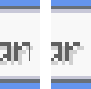
\includegraphics[height=0.15\textheight]{images/text_wrapping_comparison.png}
	\caption{Comparação de texto desenhado com carateres \emph{sem} e \emph{com} margens transparentes.}
	\label{fig:text_wrapping_comparison}
	\smallskip\small
	Esquerda: \emph{sem} margens; direita: \emph{com} margens. Note-se a linha vertical no `r' da imagem esquerda.
\end{figure}

\begin{figure}[ht]
	\centering
	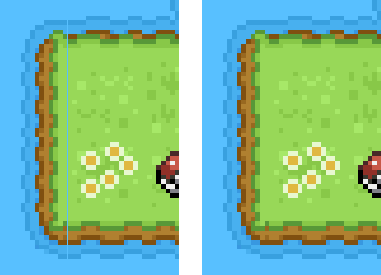
\includegraphics[height=0.23\textheight]{images/tile_wrapping_comparison.png}
	\caption{Comparação de um nível desenhado com tiles \emph{sem} e \emph{com} margens transparentes.}
	\label{fig:tile_wrapping_comparison}
	\smallskip\small
	Esquerda: \emph{sem} margens; direita: \emph{com} margens. Note-se a linha vertical azul na imagem esquerda.
\end{figure}

\subsubsection{Interface do utilizador}

As próximas secções descrevem aspetos gerais da interface do utilizador, relevantes em todo o programa.

\paragraph{Ajuste do tamanho}
\label{sec:ajustedotamanho}

Toda a interface do utilizador, ao longo de todo o programa, é capaz de se ajustar ao tamanho da janela, a qual pode ser redimensionada pelo utilizador a qualquer momento. A interface é redimensionada ao maior tamanho possível de maneira a caber na janela, e depois centrada. Isto é conseguido através das seguintes funções do módulo \haskell{Sokoban.Helper}:

\begin{haskellblock}
zoomRegionToTop     :: Rect -> Rect -> Rect
zoomRegionToCenter  :: Rect -> Rect -> Rect
zoomRegionToBottom  :: Rect -> Rect -> Rect

zoomRectToTop       :: Rect -> Rect -> Rect -> Rect
zoomRectToCenter    :: Rect -> Rect -> Rect -> Rect
zoomRectToBottom    :: Rect -> Rect -> Rect -> Rect

zoomPictureToTop    :: Rect -> Rect -> Picture -> Picture
zoomPictureToCenter :: Rect -> Rect -> Picture -> Picture
zoomPictureToBottom :: Rect -> Rect -> Picture -> Picture
\end{haskellblock}

Para mais informações sobre estas funções, cf. documentação do código.

\paragraph{Desenho de texto}

O sistema de desenho de texto da biblioteca \emph{Gloss}, o qual utiliza um tipo de letra vetorial, não permite a definição exata da posição ou do tamanho do texto. O tipo de letra não se enquadra também no estilo visual do jogo. Por estas razões, desenvolvemos o nosso próprio sistema de desenho de texto. Este sistema foi implementado no módulo \haskell{Sokoban.UI.Font}.

O texto é constituído por carateres individuais, cada um representado por uma imagem; estas imagens são carregadas, relativamente ao executável do programa, da diretoria \texttt{assets/ui/font/}. O sistema permite a definção do tamanho, alinhamento e cor do texto. Pode também ser especificada, opcionalmente, a cor da sombra do texto.

O sistema é capaz de processar o caratere \haskell{'\n'} de maneira a indicar uma mudança de linha (cf. figura \ref{fig:text}).

\begin{figure}[ht]
	\centering
	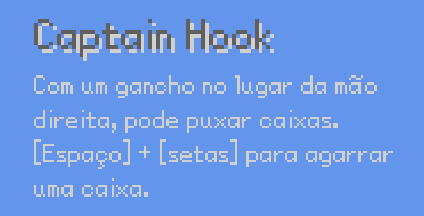
\includegraphics[height=0.15\textheight]{images/text.png}
	\caption{Texto com newlines.}
	\label{fig:text}
\end{figure}

\paragraph{Botões}

Ao longo de todo o programa, são utilizados botões interativos na interface do utilizador, os quais podem ser utilizados para efetuar ações, e.g. sair do jogo ou anular uma jogada. O utilizador pode interagir com estes botões utilizando o rato ou o teclado.

Ao colocar o cursor do rato sobre um botão, o aspeto visual deste muda. Quando o utilizador prime o botão esquerdo do rato com o cursor sobre um botão, o seu aspeto visual muda também, e quando o botão é largado, a ação associada com o botão é executada (cf. figura \ref{fig:buttons}).

\begin{figure}[ht]
	\centering
	
\includegraphics[width=0.8\textwidth]{images/buttons.png}
	\caption{Diferentes aspetos visuais de um botão.}
	\label{fig:buttons}
	\smallskip\small
	Esquerda: cursor fora do botão; centro: cursor sobre o botão; direita: cursor sobre o botão e botão esquerdo do rato premido.
\end{figure}

O utilizador pode também ativar o botão premindo a tecla que lhe foi associada.

Devido à funcionalidade do ajuste do tamanho da interface ao tamanho da janela, é necessário ter em conta essa transformação ao processar a posição do cursor. Isto é feito com recurso às mesmas funções do módulo \haskell{Sokoban.Helper} citadas na secção \ref{sec:ajustedotamanho}.

\subsubsection{Menu}

O menu incial aparece quando se inicia o jogo. Aqui encontram-se o título do jogo, um selecionador de personagem e dois botões que permitem avançar para o jogo ou sair (cf. figura \ref{fig:menu}). O utilizador pode selecionar o personagem utilizando o rato (de forma similar a interagir com um botão) ou as setas do teclado.

\begin{figure}[ht]
	\centering
	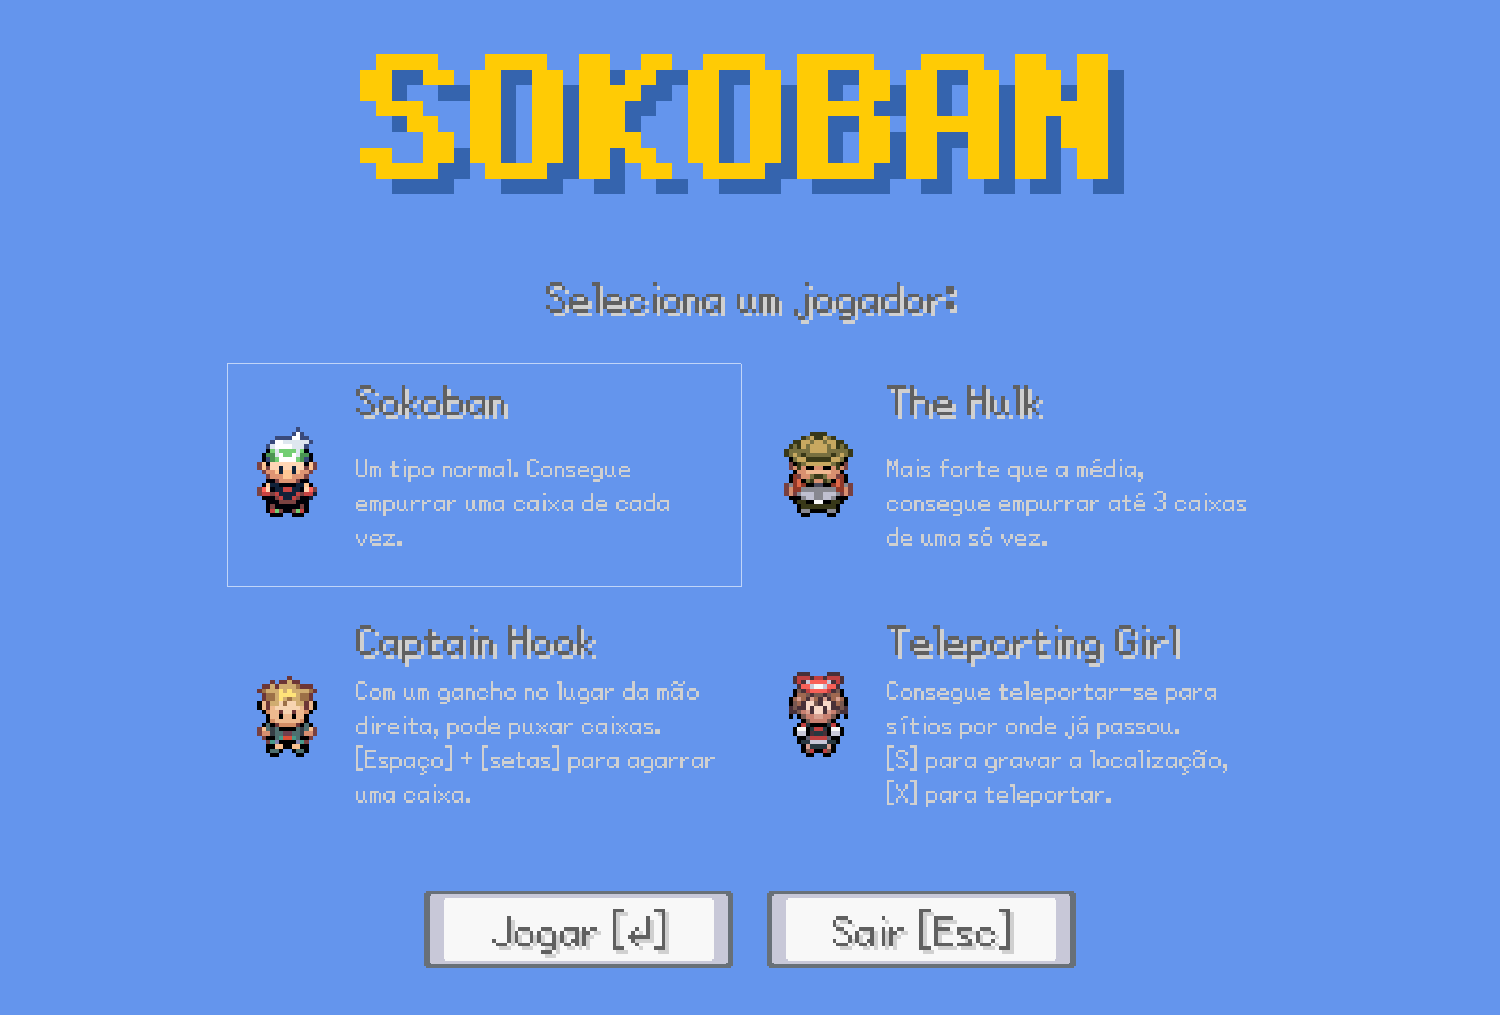
\includegraphics[width=0.9\textwidth]{images/menu.png}
	\caption{Menu inicial.}
	\label{fig:menu}
\end{figure}

O utilizador pode também regressar a este menu depois de terminar um nível, para escolher um novo personagem.

\subsubsection{Jogo}

Descreve-se agora a fase do programa na qual o utilizador resolve puzzles do jogo \textit{Sokoban}.

No topo da interface, incluiu-se um painel que mostra o número do nível atual, o número total de níveis, o número de passos efetuados no nível atual e o tempo decorrido desde o início do nível atual (cf. figura \ref{fig:game}).

Existe também, em baixo, um painel com botões que permitem controlar certos aspetos do jogo. Se o nível atual se encontra por resolver e o utilizador não desistiu, existem 3 botões, os quais permitem anular a jogada anterior, recomeçar o nível ou desistir do nível atual (cf. figura \ref{fig:game}). Quando o nível se encontra resolvido ou o utilizador desistiu, existe um botão que permite ao utilizador regressar ao menu inicial; se ainda existirem níveis por jogar, aparece também um botão que permite passar ao próximo nível.

\begin{figure}[ht]
	\centering
	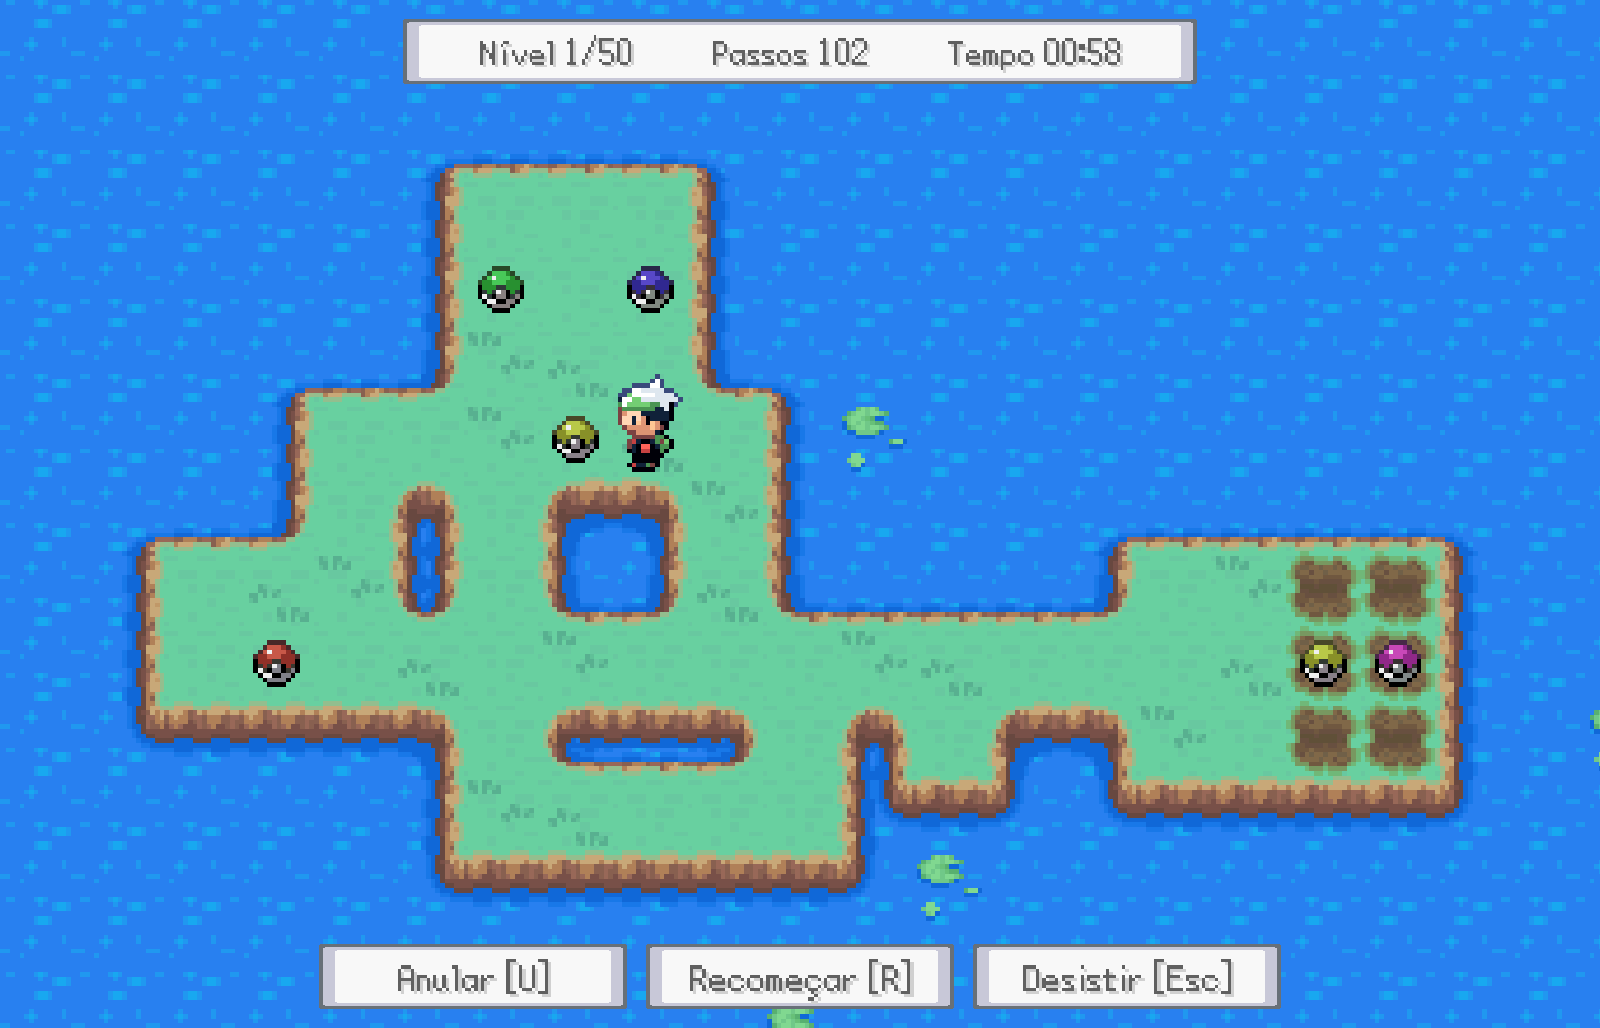
\includegraphics[width=0.9\textwidth]{images/game.png}
	\caption{Jogo.}
	\label{fig:game}
\end{figure}

\paragraph{Nível}

Para controlar o estado do puzzle e o input do utilizador, criou-se um sistema dividido em 4 módulos: \haskell{Sokoban.Game.Level}, \haskell{Sokoban.Game.Board}, \haskell{Sokoban.Game.Player} e \haskell{Sokoban.Game.Boxes}. Este sistema é responsável por armazenar e atualizar o estado do puzzle, reagir ao input do utilizador e desenhar o mapa de jogo, incluindo o personagem e as caixas.

\bigskip

O módulo \haskell{Sokoban.Game.Board} exporta tipos e funções responsáveis por gerir o tabuleiro de jogo. Este tabuleiro é estático, i.e. pode ser construído quando o nível é criado e não precisa de ser atualizado nem de reagir ao input do utilizador. Uma das suas responsabilidades é a de desenhar a imagem do tabuleiro.

\bigskip

O módulo \haskell{Sokoban.Game.Player} é principalmente responsável por gerir o aspeto gráfico do personagem, incluindo animações, e por disponibilizar um sistema que permita anular jogadas já efetuadas. A reação ao input do utilizador e a verificação das habilidades de cada personagem serão geridos pelo módulo \haskell{Sokoban.Game.Level}.

\bigskip

O módulo \haskell{Sokoban.Game.Boxes} é responsável por gerir o aspeto gráfico das caixas, incluindo animações, e por disponibilizar um sistema que permita anular ações já efetuadas sobre as caixas.

\bigskip

O módulo \haskell{Sokoban.Game.Level} junta os três módulos anteriores, sendo também acrescido da responsabilidade de reagir ao input do utilizador; é este módulo que verifica se uma ação é válida para um determinado personagem, tendo em conta as suas habilidades. É também responsável por executar, no início do nível, os comandos que devem ser executados automaticamente pelo personagem.

Quando o utilizador decide anular uma jogada, este módulo é informado e delega essa responsabilidade para os módulos \haskell{Sokoban.Game.Player} e \haskell{Sokoban.Game.Boxes}. No caso de o utilizador querer recomeçar o nível, este módulo é responsável por anular todas as jogadas possíveis consecutivamente.

\subsection{Testes}

O programa, pela seu natureza, não permite a utilização de testes que verifiquem pares de input-output sobre o programa (black-box testing). Assim, para testar a validade do programa, foram elaborados testes de dois tipos:

\begin{itemize}
	\item Verificação de pares de input-output sobre funções individuais: através da utilização da biblioteca \textit{HUnit}\footnote{\url{http://hunit.sourceforge.net}}, definiram-se vários testes de verificação da correspondência do output de várias funções com determinados inputs.
	\item Verificação de propriedades de funções: recorrendo à biblioteca \textit{QuickCheck}\footnote{\url{https://github.com/nick8325/quickcheck}}, criaram-se vários testes para a verificação de diversas propriedades de várias funções.
\end{itemize}

No total, definiram-se 61 testes através da biblioteca \textit{HUnit} e 17 testes através da biblioteca \textit{QuickCheck}. O programa passa em todos.

\section{Conclusão}

Neste documento foi descrito o processo de desenvolvimento do projeto realizado no âmbito da Unidade Curricular de Laboratórios de Informática I, tendo sido focadas as tarefas E e F. Descreveu-se, para estes dois problemas, o processo de conceção da solução, a sua implementação e os testes sobre estes efetuados.

Os programas desenvolvidos como solução aos problemas propostos pelo enunciado foram submetidos na plataforma \textit{mooshak}, tendo todos eles passado em todos os testes.

Em última análise, consideramos que os objetivos definidos foram cumpridos.

\appendix

\newpage
\section{Tarefa E - Tipos e funções auxiliares}
\label{app:tarefaEaux}

\haskellfile{shortTarefaE.hs}

\newpage
\section{Tarefa F - Hierarquia de módulos}
\label{app:tarefaFmodulos}

\global\pdfpageattr\expandafter{\the\pdfpageattr/Rotate 90}

\begin{figure}[!ht]
	\centering
	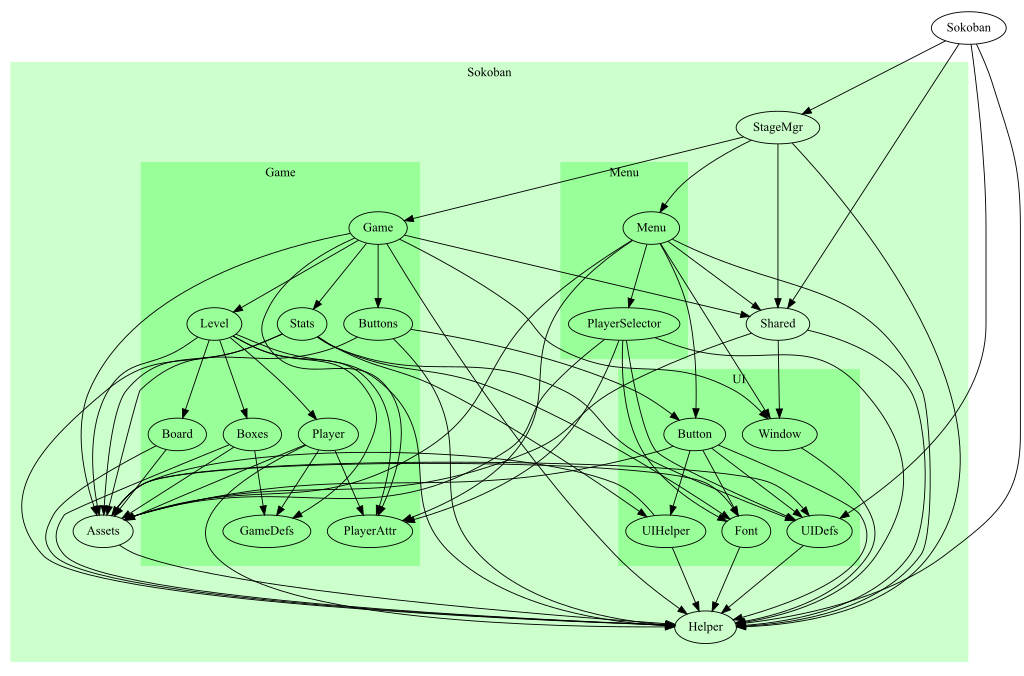
\includegraphics[angle=90,width=0.6\textheight]{images/modules.png}
	\caption{Hierarquia de módulos.}
\end{figure}

\end{document}
